\documentclass{article}
\usepackage{mainPoly}

\title{Ensembles de nombres : arithmétique, intervalle}
\date{}
\author{Seconde 9}

\begin{document}
\maketitle

\section{Introduction}
\begin{tcolorbox}
\begin{definition}
Un \textbf{ensemble de nombres} est une collection de nombres partageant la même nature.
\end{definition}
\end{tcolorbox}
\begin{example}
On peut parler de l'ensemble des nombres renvoyés par un dé, ou l'ensemble des âges des élèves de la classe de seconde 9, ou encore l'ensemble de tous les prix affichés dans un supermarché.
\end{example}
\textbf{Par la suite, nous allons nous intéresser à différents ensembles classiques de nombres, et voir la façon dont sont étudiés les nombres associés.}
\section{Nombres entiers}
\subsection{Ensembles}
\begin{definition}
\hfill
\begin{itemize}
\item On note $\N$ l'ensemble des nombres entiers \textbf{Naturels} : il s'agit de tous les entiers plus grands ou égaux à $0$, comme $0$; $1$; $2$ \dots
\item On note $\Z$ l'ensemble des nombres entiers \textbf{relatifs} : il s'agit des entiers supérieurs, inférieurs ou égaux à \textbf{Zéro}, comme $-2$; $-1$; $0$; $1$; $2$ \dots
\end{itemize}
\end{definition}
\begin{definition}
\hfill

Pour dire qu'un nombre $n$ est un entier naturel, on écrit $n \in \N$. Cela se lit \emph{\og $n$ appartient à $\N$ \fg}.

Pour dire qu'un nombre $n$ est un entier relatif, on écrit $n \in \Z$. Cela se lit \emph{\og $n$ appartient à $\Z$ \fg}.
\end{definition}
\begin{example}
Vrai ou faux ? Répondre dans chacun des cas suivants.
\begin{enumquestions}
\begin{minipage}{0.45\textwidth}
\item $6 \in \N$ \answersline
\item $-9 \in \N$ \answersline
\item $-4 \in \Z$ \answersline
\end{minipage}
\hfill
\begin{minipage}{0.45\textwidth}
\item $12 \in \Z$ \answersline        
\item $5 \notin \N$ \answersline
\item $-8 \notin \N$ \answersline
\end{minipage}
\end{enumquestions}
\end{example}
\begin{proposition}
Tout nombre entier naturel est un nombre entier relatif. Du point des ensembles, cette proposition se note $\N \subset \Z$.
\end{proposition}
\begin{example}
Placer les nombres suivants dans le schéma : $5$; $2$; $-10$; $0$ et $-6$.
\begin{center}
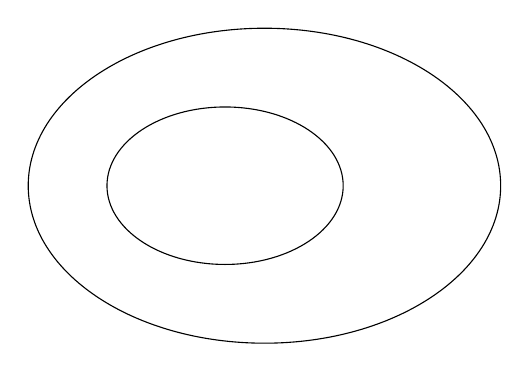
\begin{tikzpicture}
\draw (0,0) ellipse (3 and 2);
\draw (-0.5,0) ellipse (1.5 and 1);
\draw (2.5,0) node {$\Z$};
\draw (0.5,0) node {$\N$};
\end{tikzpicture}
\end{center}
\end{example}
\newpage
\subsection{Arithmétique}
\textbf{Nous travaillons avec les nombres de $\Z$. Dans ce contexte, on ne considère pas les divisions réelles, ni les fractions.}
\begin{tcolorbox}
\begin{definition}
Soit $a$ et $b$ deux entiers relatifs.
\begin{itemize}
\item $a$ est un \textbf{multiple} de $b$ si et seulement si il existe $k \in \Z$ tel que $a = k \times b$.
\item $b$ est un \textbf{diviseur} de $a$ si et seulement si il existe $k \in \Z$ tel que $a = k \times b$.
\end{itemize}
\end{definition}
\end{tcolorbox}
\begin{example}
\hfill
\begin{itemize}
\item Le nombre $10$ est un multiple de $2$ : en effet, il existe un nombre entier relatif $k = 5$ tel que $10 = k \times 2$.
\item Le nombre $7$ est un diviseur de $-28$ : en effet, il existe un nombre entier relatif $k = -4$ tel que $28 = k \times 7$.
\end{itemize}
\end{example}
\begin{example}
\hfill

Le nombre $36$ est-il un multiple de $3$ ? Justifier. \answersline

Le nombre $-8$ est-il un diviseur de $128$ ? Justifier. \answersline
\end{example}

\begin{remark}
Tout nombre est divisible par $0$. Ou, de façon équivalente, $0$ est le multiple de n'importe quel nombre. 
\end{remark}

\begin{proposition}
La somme de deux multiples de $a$ est un multiple de $a$.
\end{proposition}
\begin{proof}
\hfill
\vspace*{0.5cm}
\hfill
\emptybox{7cm}
\end{proof}
\newpage
\begin{definition}
\hfill
\begin{itemize}
\item Un nombre entier relatif est \textbf{pair} si et seulement s'il est divisible par $2$.
\item Un nombre entier relatif est \textbf{impair} si et seulement s'il n'est pas pair. 
\end{itemize}
\end{definition}
\begin{example}
\hfill

Le nombre $12$ est pair : en effet, il est divisible par $2$, car $12 = 2 \times 6$.

Le nombre $-27$ est impair : en effet, il n'est pas pair, car il n'existe pas d'entier relatif $k$ vérifiant $-27 = 2 \times k$.
\end{example}

\begin{proposition}
Un nombre $n \in \Z$ est impair si et seulement si il existe $p \in \Z$ tel que $n = 2 \times p + 1$.
\end{proposition}

\begin{proposition}
Soit $x$ et $y$ deux entiers relatifs. Alors, les tableaux suivants décrivent la parité de $x + y$ et de $x \times y$.
\vspace*{0.5cm}

\begin{minipage}{0.30\textwidth}
\begin{tabular}{|c|c|c|}
\hline
$x + y$&$y$ pair&$y$ impair\\
\hline
$x$ pair&pair& impair\\
\hline
$x$ impair& impair& pair\\
\hline
\end{tabular}    
\end{minipage}
\hfill
\begin{minipage}{0.30\textwidth}
\begin{tabular}{|c|c|c|}
\hline
$x \times y$&$y$ pair&$y$ impair\\
\hline
$x$ pair&pair& pair\\
\hline
$x$ impair& pair& impair\\
\hline
\end{tabular}    
\end{minipage}
\hfill
\begin{minipage}{0.30\textwidth}
\begin{tabular}{|c|c|c|}
\hline
$x^2$&$x$ pair&$x$ impair\\
\hline
&pair& impair\\
\hline
\end{tabular}    
\end{minipage}
\end{proposition}
\begin{proof}
On démontre ici uniquement la propriété suivante : si $x$ est un entier relatif impair, alors $x^2$ est impair.
\vspace*{0.5cm}

\emptybox{7cm}
\end{proof}

\newpage
\begin{tcolorbox}
\begin{definition}
Un nombre entier naturel $n \in \N$ est \textbf{premier} si et seulement si il admet exactement deux diviseurs positifs : $1$ et lui-même. 
\end{definition}
\end{tcolorbox}
\begin{remark}
\hfill
\begin{itemize}
\item Traditionnellement, un nombre premier est \textbf{positif} : on ne s'intéresse qu'aux entiers naturels dans ce cadre.
\item Le nombre $1$ n'est \textbf{\textsc{pas}} premier : il n'admet qu'un seul diviseur positif. 
\end{itemize}
\end{remark}
\begin{example}
Les nombres suivants sont premiers: $2; 3; 5; 7; 11; 13; 17; 19 \dots$
\end{example}
\begin{proposition}
Tout entier naturel supérieur ou égal à $2$ peut s'écrire comme un produit de nombres premiers. 
\end{proposition}
\begin{example}
\hfill
\begin{itemize}
\item $18 = 2 \times 3 \times 3$
\item $68 =$ \answersline 
\item $132 =$ \answersline
\item $85 =$ \answersline
\end{itemize}
\end{example}
\begin{example}
On peut écrire des fractions sous forme irréductible à l'aide de la décomposition du numérateur et du dénominateur en produit de facteurs premiers.
\begin{itemize}
\item $\dfrac{500}{75} = \dfrac{2 \times 2 \times 5 \times \cancel{5} \times \cancel{5}}{3 \times \cancel{5} \times \cancel{5}} = \dfrac{2 \times 2 \times 5}{3} = \dfrac{20}{3}$
\item $\dfrac{126}{24} =$ \answersline
\item $\dfrac{3}{45} =$ \answersline
\end{itemize}
\end{example}

\newpage
\section{Nombres rationels}
\subsection{Ensembles}
\begin{definition}
\hfill
\begin{itemize}
\item On note $\D$ l'ensemble des \textbf{nombres décimaux}, c'est-à-dire l'ensemble des nombres dont l'écriture décimale est finie (nombre fini de chiffres après la virgule).
\item On note $\Q$ l'ensemble des \textbf{nombres rationels}, c'est-à-dire l'ensemble des nombres pouvant s'écrire sous la forme d'une fraction d'entiers
\begin{equation*}
\dfrac{a}{b}
\end{equation*}
avec $a \in \Z$, $b \in \N$ et $n \neq 0$.
\end{itemize}
\end{definition}
\begin{example}
Les nombres suivants sont des nombres décimaux : $1,23$; $2$; $-3,4$ \dots

Les nombres suivants sont des nombres rationels :
$1,23$; $\dfrac{4}{2}$; $\dfrac{1}{3}$ \dots
\end{example}
\begin{proposition}
Tout nombre $x \in \D$ est de la forme
\begin{equation*}
x = \dfrac{a}{10^k}
\end{equation*}
tel que $a \in Z$ et $k \in \N$.
\end{proposition}
\begin{remark}
\hfill
\begin{itemize}
\item Cette proposition nous permet d'affirmer que tout nombre décimal est un nombre rationel. Cela s'écrit $\D \subseteq \Q$.
\item Tout entier relatif est un nombre décimal. On en déduit que tout entier relatif est un nombre rationel. En effet, si $x \in \Z$, alors $x = \dfrac{x}{1} = \dfrac{x}{10^0}$. 
\end{itemize}
\end{remark}
\begin{example}
Compléter le schéma suivant en mettant chaque nombre dans l'ensemble le plus petit le contenant :
$2$; $-4,3$; $\dfrac{1}{7}$; $\dfrac{-10}{2}$; $21,333\dots$; $0$; $\dfrac{10}{25}$.
\begin{center}
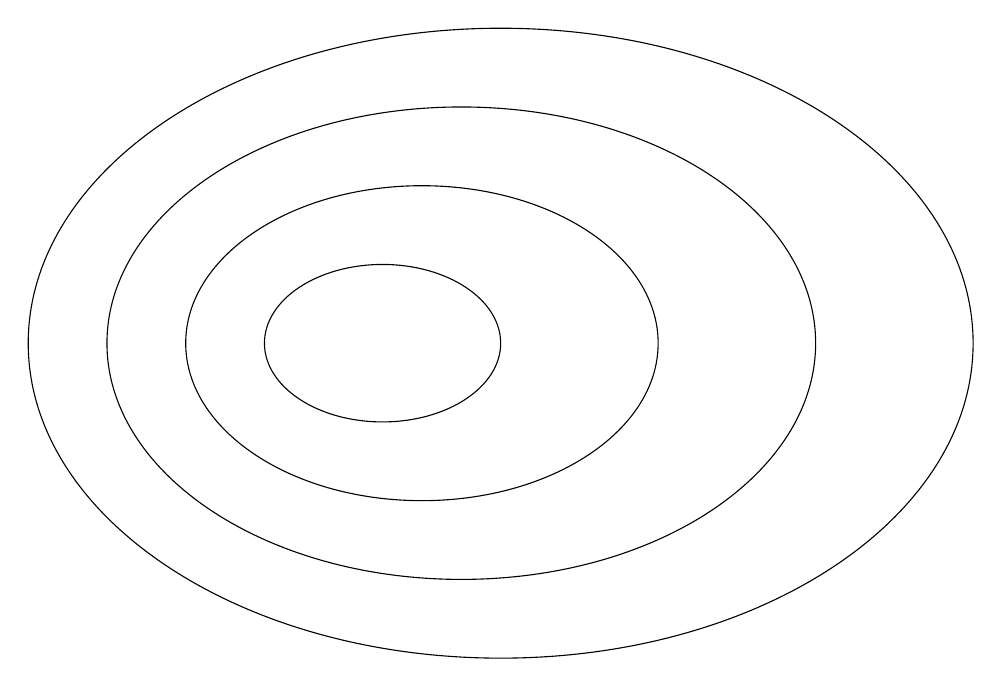
\begin{tikzpicture}
\draw (1,0) ellipse (6 and 4);
\draw (0.5,0) ellipse (4.5 and 3);
\draw (0,0) ellipse (3 and 2);
\draw (-0.5,0) ellipse (1.5 and 1);
\draw (6.5,0) node {$\Q$};
\draw (4.5,0) node {$\D$};
\draw (2.5,0) node {$\Z$};
\draw (0.5,0) node {$\N$};
\end{tikzpicture}    
\end{center}
\end{example}
\newpage
\subsection{Formes irréductibles}
\begin{proposition}
Soit $x \in \Q$. Alors $x$ est de la forme
\begin{equation*}
x = \dfrac{a}{b}
\end{equation*}
avec $a$ et $b$ deux entiers dont le seul diviseur positif en commun est $1$. On dit que cette fraction est \textbf{irréductible}.
\end{proposition}
\begin{example}
\hfill
\begin{enumquestions}
\item La fraction $\dfrac{67}{15}$ est-elle irréductible ? \answersline
\item La fraction $\dfrac{789}{456}$ est-elle irréductible ? \answersline
\end{enumquestions}
\end{example}
\begin{proposition}
\label{prop : decimal_condition}
Soit $x$ un nombre rationel dont la forme irréductible est donnée par $\dfrac{a}{b}$. Si la décomposition en facteurs premier de $b$ ne fait qu'apparaître des $2$ et des $5$, alors $x$ est un nombre décimal.
\end{proposition}
\begin{example}
\hfill
\begin{enumquestions}
\item $\dfrac{3}{50}$ est-il décimal ? \answersline
\item $\dfrac{8}{12}$ est-il décimal ? \answersline
\item $\dfrac{45}{12}$ est-il décimal ? \answersline
\end{enumquestions}
\end{example}
\begin{proposition}
$\dfrac{1}{3}$ n'est pas décimal.
\end{proposition}
\begin{proof}
La démonstration suivante n'utilise pas la proposition \ref{prop : decimal_condition}.
\vspace*{0.5cm}

\emptybox{8cm}
\end{proof}

\newpage

\section{Nombres réels, intervalles}
\subsection{Ensemble $\R$}
\begin{remark}
Certains nombres ne sont des éléments d'aucun des ensembles mentionnés. En particulier, certains nombres ne sont pas rationnels. C'est le cas de $\pi$ ou de $\sqrt{2}$. On dit donc qu'ils sont \textbf{irrationels}.
\end{remark}
\begin{tcolorbox}
\begin{definition}
On note $\R$ l'ensemble des nombres \textbf{réels}.
\end{definition}
\end{tcolorbox}
\begin{tcolorbox}
\begin{proposition}
Les différents ensembles de nombres vu précédemment vérifient les inclusions suivantes :
\begin{equation*}
\N \subseteq \Z \subseteq \D \subseteq \Q \subseteq \R
\end{equation*}
\end{proposition}
\end{tcolorbox}
\begin{example}
Intégrer dans le schéma ci-dessous les nombres suivants : $2$; $-3$; $0,5$; $\dfrac{4}{3}$; $\pi$; $\sqrt{2}$; $\dfrac{27}{16}$; $-1,666\dots{}$


\begin{center}
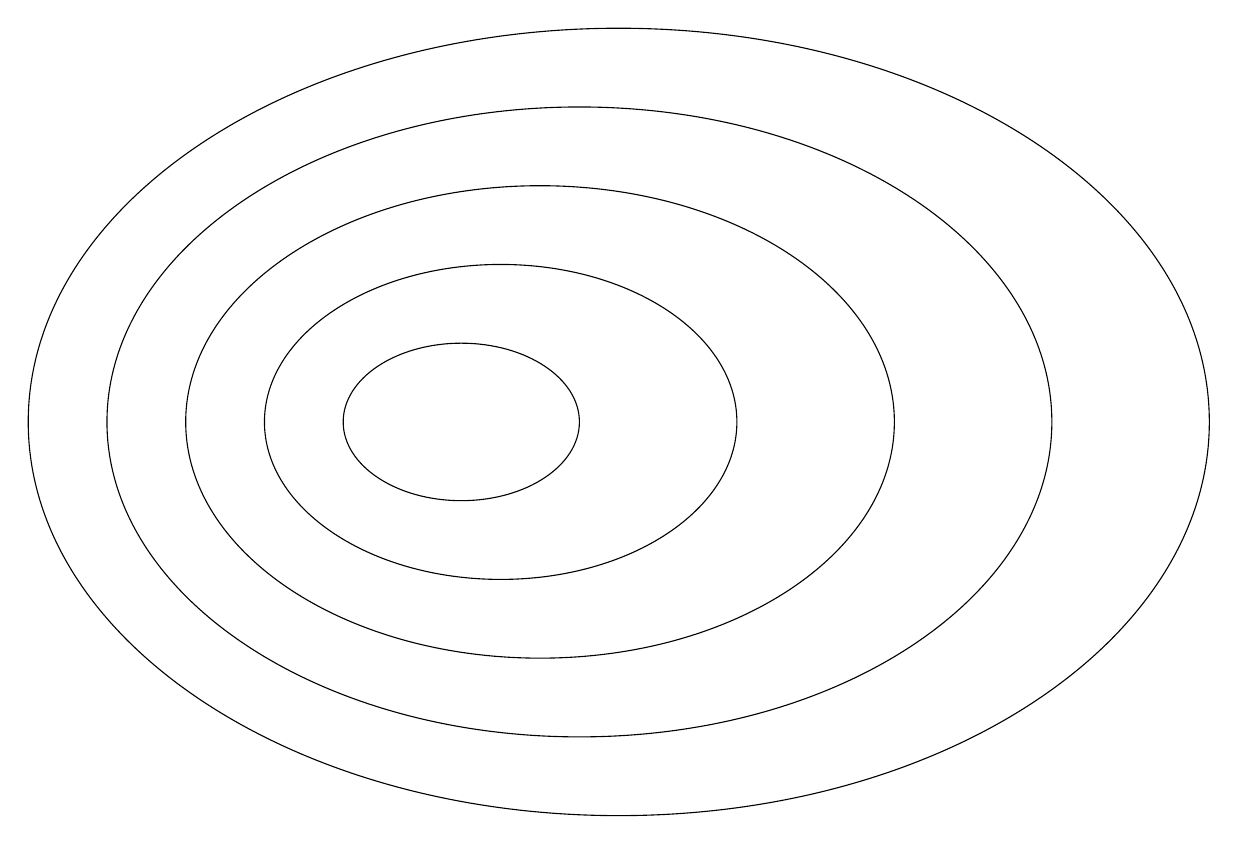
\begin{tikzpicture}
\draw (1.5,0) ellipse (7.5 and 5);
\draw (1,0) ellipse (6 and 4);
\draw (0.5,0) ellipse (4.5 and 3);
\draw (0,0) ellipse (3 and 2);
\draw (-0.5,0) ellipse (1.5 and 1);
\draw (8.5,0) node {$\R$};
\draw (6.5,0) node {$\Q$};
\draw (4.5,0) node {$\D$};
\draw (2.5,0) node {$\Z$};
\draw (0.5,0) node {$\N$};
\end{tikzpicture} 
\end{center}
\end{example}
\begin{proposition}
Pour représenter l'ensemble des réel, on utilise une droite graduée nommée la \textbf{droite des réels}. Chaque point de la droite correspond à un nombre réel, et chaque nombre réel est associé à un point de cette droite.
\end{proposition}
\begin{center}
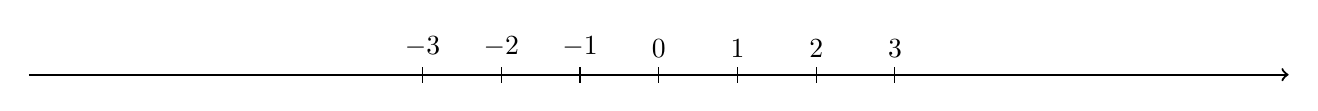
\begin{tikzpicture}
\draw[->, thick] (-8,0) -- (8,0);
\draw (0,-0.1) -- (0,0.1) node[above] {$0$};
\draw (1,-0.1) -- (1,0.1) node[above] {$1$};
\draw (2,-0.1) -- (2,0.1) node[above] {$2$};
\draw (3,-0.1) -- (3,0.1) node[above] {$3$};
\draw (-1,-0.1) -- (-1,0.1) node[above] {$-1$};
\draw (-2,-0.1) -- (-2,0.1) node[above] {$-2$};
\draw (-3,-0.1) -- (-3,0.1) node[above] {$-3$};
\end{tikzpicture}
\end{center}
\begin{example}
Placer approximativement sur cette droite les points associés aux nombres utlisés dans l'exemple précédent.
\end{example}

\newpage

\subsection{Intervalles de $\R$}
\begin{tcolorbox}
\begin{definition}
Soit $a,b$ deux nombres réels tels que $a < b$.
\begin{itemize}
\item L'intervalle $[a;b]$ est l'ensemble de tous les nombres réels $x$ vérifiant $a \leq x \leq b$. 
\item L'intervalle $]a;b]$ est l'ensemble de tous les nombres réels $x$ vérifiant $a < x \leq b$. 
\item L'intervalle $[a;b[$ est l'ensemble de tous les nombres réels $x$ vérifiant $a \leq x < b$. 
\item L'intervalle $]a;b[$ est l'ensemble de tous les nombres réels $x$ vérifiant $a < x < b$. 
\end{itemize}
\end{definition}
\end{tcolorbox}
\begin{remark}
Un intervalle décrit donc un ensemble de nombres compris entre deux bornes. Le sens des crochets indique si une borne est comprise ou non dans l'intervalle.
\end{remark}
\begin{example}
Pour chacune des phrases suivantes, donner la notation de l'intervalle correspondant :
\begin{enumquestions}
\item Les nombres compris entre $2$ (inclus) et $5$ (inclus) : $[2;5]$
\item Les nombres compris entre $4$ (exclus) et $12$ (inclus) : \answersline
\item Tous les nombres supérieurs ou égaux à $-10$ et inférieurs strictement à $-5$ : \answersline
\item Tous les nombres positifs non nuls inférieurs strictement à $113$ : \answersline
\end{enumquestions}
\end{example}
\begin{tcolorbox}
\begin{definition}
Soit $a$ un nombre réel.
\begin{itemize}
\item L'intervalle $[a;+\infty[$ est l'ensemble des nombres $x$ vérifiant $a \leq x$.
\item L'intervalle $]a;+\infty[$ est l'ensemble des nombres $x$ vérifiant $a < x$.
\item L'intervalle $]-\infty; a]$ est l'ensemble des nombres $x$ vérifiant $x \leq a$.
\item L'intervalle $]-\infty; a[$ est l'ensemble des nombres $x$ vérifiant $x < a$.
\end{itemize}
\end{definition}
\end{tcolorbox}
\begin{remark}
\hfill

\begin{itemize}
\item Avec les symboles $- \infty$ (\og $-$ l'infini \fg) et $+ \infty$ (\og $+$ l'infini \fg), le crochet est toujours ouvrant.
\item En théorie, $\R = ]-\infty; +\infty[$.
\end{itemize}
\end{remark}
\begin{remark}
Les intervalles se représentent comme des portions continues de la droite des réels. On ajoute des crochets identiques à celui de l'intervalle.

On a représenté $[1;3]$ sur la droite des réels représentée ci-desouss. 

Représenter $]-3;-1[$.
\begin{center}
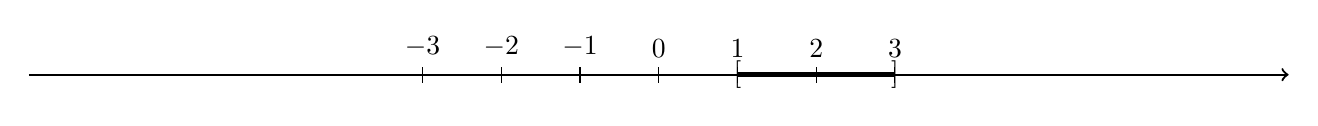
\begin{tikzpicture}
\draw[->, thick] (-8,0) -- (8,0);
\draw (0,-0.1) -- (0,0.1) node[above] {$0$};
\draw (1,-0.1) -- (1,0.1) node[above] {$1$};
\draw (2,-0.1) -- (2,0.1) node[above] {$2$};
\draw (3,-0.1) -- (3,0.1) node[above] {$3$};
\draw (-1,-0.1) -- (-1,0.1) node[above] {$-1$};
\draw (-2,-0.1) -- (-2,0.1) node[above] {$-2$};
\draw (-3,-0.1) -- (-3,0.1) node[above] {$-3$};
\draw[ultra thick] (1,0) node {$[$} -- (3,0) node {$]$};
\end{tikzpicture}
\end{center}
\end{remark}
\end{document}

